\documentclass[tikz,border=2pt]{standalone}

\usepackage{pgfplots}
\usepgfplotslibrary{groupplots}
\usetikzlibrary{arrows.meta}
\pgfplotsset{compat=1.18}
\definecolor{cbBlue}{HTML}{0072B2}
\definecolor{cbOrange}{HTML}{D55E00}
\definecolor{cbGreen}{HTML}{009E73}
\definecolor{cbPurple}{HTML}{CC79A7}
\definecolor{cbSky}{HTML}{56B4E9}
\definecolor{cbGold}{HTML}{E69F00}
\pgfplotsset{
  paperaxis/.style={
    axis line style={black!65,line width=0.45pt},
    tick style={black!65,line width=0.45pt},
    tick label style={font=\footnotesize},
    label style={font=\small},
    title style={font=\small\bfseries,yshift=-1pt},
    grid=major,
    grid style={black!10,line width=0.35pt},
    line width=1.05pt,
    mark size=1.8pt,
  }
}

\begin{document}
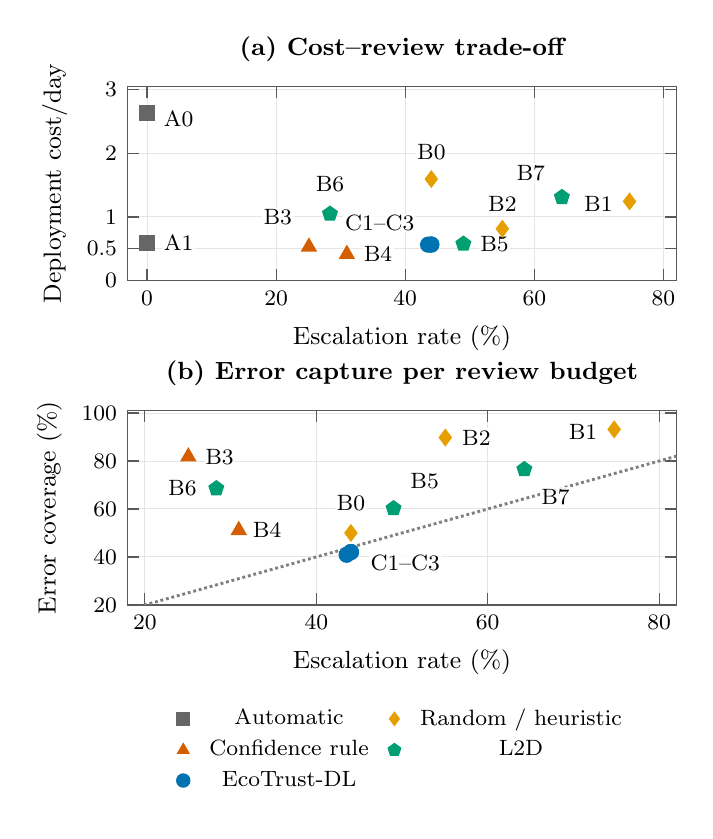
\begin{tikzpicture}
\begin{groupplot}[
  group style={group size=1 by 2,vertical sep=1.65cm},
  paperaxis,width=8.55cm,height=4.05cm,
]
\nextgroupplot[
  title={(a) Cost--review trade-off},
  xmin=-3,xmax=82,ymin=0,ymax=3.05,
  xlabel={Escalation rate (\%)},ylabel={Deployment cost/day},
  xtick={0,20,40,60,80},ytick={0,0.5,1,2,3},
  legend to name=methodlegend,
  legend columns=2,
  legend style={font=\footnotesize,draw=none,column sep=5pt},
]
\addplot[only marks,black!60,mark=square*,mark size=2.4pt] coordinates {(0.000,2.6270) (0.000,0.5960)};
\addlegendentry{Automatic}
\addplot[only marks,cbGold,mark=diamond*,mark size=2.4pt] coordinates {(44.040,1.5940) (74.750,1.2440) (55.050,0.8140)};
\addlegendentry{Random / heuristic}
\addplot[only marks,cbOrange,mark=triangle*,mark size=2.4pt] coordinates {(25.080,0.5310) (30.960,0.4160)};
\addlegendentry{Confidence rule}
\addplot[only marks,cbGreen,mark=pentagon*,mark size=2.4pt] coordinates {(49.010,0.5770) (28.340,1.0480) (64.270,1.3100)};
\addlegendentry{L2D}
\addplot[only marks,cbBlue,mark=*,mark size=2.4pt] coordinates {(44.040,0.5670) (44.040,0.5670) (43.540,0.5650)};
\addlegendentry{EcoTrust-DL}
\node[font=\footnotesize,anchor=west,fill=white,fill opacity=.84,text opacity=1,inner sep=.6pt] at ([xshift=5pt,yshift=-2pt]axis cs:0.000,2.6270) {A0};
\node[font=\footnotesize,anchor=west,fill=white,fill opacity=.84,text opacity=1,inner sep=.6pt] at ([xshift=5pt,yshift=0pt]axis cs:0.000,0.5960) {A1};
\node[font=\footnotesize,anchor=south,fill=white,fill opacity=.84,text opacity=1,inner sep=.6pt] at ([xshift=0pt,yshift=6pt]axis cs:44.040,1.5940) {B0};
\node[font=\footnotesize,anchor=east,fill=white,fill opacity=.84,text opacity=1,inner sep=.6pt] at ([xshift=-5pt,yshift=-1pt]axis cs:74.750,1.2440) {B1};
\node[font=\footnotesize,anchor=south,fill=white,fill opacity=.84,text opacity=1,inner sep=.6pt] at ([xshift=0pt,yshift=5pt]axis cs:55.050,0.8140) {B2};
\node[font=\footnotesize,anchor=south east,fill=white,fill opacity=.84,text opacity=1,inner sep=.6pt] at ([xshift=-5pt,yshift=7pt]axis cs:25.080,0.5310) {B3};
\node[font=\footnotesize,anchor=west,fill=white,fill opacity=.84,text opacity=1,inner sep=.6pt] at ([xshift=5pt,yshift=0pt]axis cs:30.960,0.4160) {B4};
\node[font=\footnotesize,anchor=west,fill=white,fill opacity=.84,text opacity=1,inner sep=.6pt] at ([xshift=5pt,yshift=0pt]axis cs:49.010,0.5770) {B5};
\node[font=\footnotesize,anchor=south,fill=white,fill opacity=.84,text opacity=1,inner sep=.6pt] at ([xshift=0pt,yshift=7pt]axis cs:28.340,1.0480) {B6};
\node[font=\footnotesize,anchor=south east,fill=white,fill opacity=.84,text opacity=1,inner sep=.6pt] at ([xshift=-5pt,yshift=5pt]axis cs:64.270,1.3100) {B7};
\node[font=\footnotesize,anchor=south east,fill=white,fill opacity=.84,text opacity=1,inner sep=.6pt] at ([xshift=-5pt,yshift=4pt]axis cs:44.040,0.5670) {C1--C3};

\nextgroupplot[
  title={(b) Error capture per review budget},
  xmin=18,xmax=82,ymin=20,ymax=101,
  xlabel={Escalation rate (\%)},ylabel={Error coverage (\%)},
  xtick={20,40,60,80},ytick={20,40,60,80,100},
]
\addplot[black!50,densely dotted,domain=18:82,samples=2] {x};
\addplot[only marks,cbGold,mark=diamond*,mark size=2.4pt] coordinates {(44.040,50.0000) (74.750,93.1800) (55.050,89.7700)};
\addplot[only marks,cbOrange,mark=triangle*,mark size=2.4pt] coordinates {(25.080,81.8200) (30.960,51.1400)};
\addplot[only marks,cbGreen,mark=pentagon*,mark size=2.4pt] coordinates {(49.010,60.2300) (28.340,68.5600) (64.270,76.5200)};
\addplot[only marks,cbBlue,mark=*,mark size=2.4pt] coordinates {(44.040,42.0500) (44.040,42.0500) (43.540,40.9100)};
\node[font=\footnotesize,anchor=south,fill=white,fill opacity=.84,text opacity=1,inner sep=.6pt] at ([xshift=0pt,yshift=7pt]axis cs:44.040,50.0000) {B0};
\node[font=\footnotesize,anchor=east,fill=white,fill opacity=.84,text opacity=1,inner sep=.6pt] at ([xshift=-5pt,yshift=-1pt]axis cs:74.750,93.1800) {B1};
\node[font=\footnotesize,anchor=west,fill=white,fill opacity=.84,text opacity=1,inner sep=.6pt] at ([xshift=5pt,yshift=0pt]axis cs:55.050,89.7700) {B2};
\node[font=\footnotesize,anchor=west,fill=white,fill opacity=.84,text opacity=1,inner sep=.6pt] at ([xshift=5pt,yshift=0pt]axis cs:25.080,81.8200) {B3};
\node[font=\footnotesize,anchor=west,fill=white,fill opacity=.84,text opacity=1,inner sep=.6pt] at ([xshift=4pt,yshift=0pt]axis cs:30.960,51.1400) {B4};
\node[font=\footnotesize,anchor=south west,fill=white,fill opacity=.84,text opacity=1,inner sep=.6pt] at ([xshift=5pt,yshift=6pt]axis cs:49.010,60.2300) {B5};
\node[font=\footnotesize,anchor=east,fill=white,fill opacity=.84,text opacity=1,inner sep=.6pt] at ([xshift=-6pt,yshift=0pt]axis cs:28.340,68.5600) {B6};
\node[font=\footnotesize,anchor=north west,fill=white,fill opacity=.84,text opacity=1,inner sep=.6pt] at ([xshift=5pt,yshift=-6pt]axis cs:64.270,76.5200) {B7};
\node[font=\footnotesize,anchor=west,fill=white,fill opacity=.84,text opacity=1,inner sep=.6pt] at ([xshift=6pt,yshift=-4pt]axis cs:44.040,42.0500) {C1--C3};
\end{groupplot}
\node[anchor=north] at ([yshift=-1.05cm]group c1r2.south) {\pgfplotslegendfromname{methodlegend}};
\end{tikzpicture}
\end{document}
